% !TeX root = ../main.tex

\chapter{系统详细设计与实现}

系统的详细设计主要是对概要设计中各个功能模块的实现细节进行阐述,给出具体的设计方案.本章节将分别对模拟器四个主要功能模块的具体设计和实现细节进行阐述和说明.

\section{指令集模块的实现}

指令集模块主要实现了两个功能,指令集功能函数的翻译,以及解码器对指令列表的解析和注册.

对应单条汇编指令的取值,译码,执行过程,模拟器从PC地址读取一条32位的汇编指令,通过解码器进行解码,找到对应的功能函数,然后执行该功能函数.核心的数据结构就是指令类insn\_t,除了包含32位的uint数据成员来保存指令内容,还定义了一系列的接口,方便读取RISC-V指令格式所定义的指令码,寄存器,立即数等的位域信息.下面详细介绍模拟器对于指令类数据结构的定义和实现.
\begin{figure}[h]
    \centering
    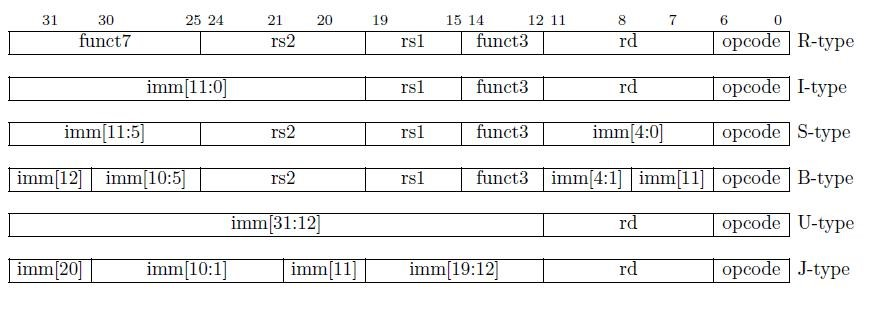
\includegraphics[width=1.0\textwidth]{insn-type.jpg}
    \caption{RISC-V32I 指令格式}
    \label{fig:insn-type}
\end{figure}
由前面的章节可以知道,RISC-V汇编指令的格式是非常明晰的,图~\ref{fig:insn-type}展示了RISC-V32I所包含的全部六种指令类型的格式。在实际编码过程中,编码位置的安排都是有意义的。例如3个寄存器索引号在不同指令格式中的编码位置是永远不变的,Rd在bit 7-11,rs1在bit 15-19,rs2在bit 20-24。即使有些指令中可能没有用到部分寄存器,比如第二个指令类型I-type中没有rs2,但是rs1和rd的索引号也在对应的位置上。又例如在S-type里funct3在bit 12-14,与在R-type中的位置一致。Opcode是所有指令格式都有的,而且位置不变,永远都是bit 0-6。


所以在指令类insn\_t中可以定义统一的接口来获取RISC-V指令中的位域信息.代码片段如下:
\begin{lstlisting}
typedef quint64 insn_bits_t;
class insn_t
{
public:
    insn_t() = default;
    insn_t(insn_bits_t bits) : b(bits) {}
    insn_bits_t bits() { return b; }
    int length() { return insn_length(b); }
    int64_t i_imm() { return int64_t(b) >> 20; }
    int64_t s_imm() { return x(7, 5) + (xs(25, 7) << 5); }
    int64_t sb_imm() { return (x(8, 4) << 1) + (x(25,6) << 5) + (x(7,1) << 11) + (imm_sign() << 12); }
    int64_t u_imm() { return int64_t(b) >> 12 << 12; }
    int64_t uj_imm() { return (x(21, 10) << 1) + (x(20, 1) << 11) + (x(12, 8) << 12) + (imm_sign() << 20); }
    quint64 rd() { return x(7, 5); }
    quint64 rs1() { return x(15, 5); }
    quint64 rs2() { return x(20, 5); }
    quint64 rs3() { return x(27, 5); }
    quint64 rm() { return x(12, 3); }
    quint64 csr() { return x(20, 12); }

    int64_t rvc_imm() { return x(2, 5) + (xs(12, 1) << 5); }
    int64_t rvc_zimm() { return x(2, 5) + (x(12, 1) << 5); }
    int64_t rvc_addi4spn_imm() { return (x(6, 1) << 2) + (x(5, 1) << 3) + (x(11, 2) << 4) + (x(7, 4) << 6); }
    int64_t rvc_addi16sp_imm() { return (x(6, 1) << 4) + (x(2, 1) << 5) + (x(5, 1) << 6) + (x(3, 2) << 7) + (xs(12, 1) << 9); }
    int64_t rvc_lwsp_imm() { return (x(4, 3) << 2) + (x(12, 1) << 5) + (x(2, 2) << 6); }
    int64_t rvc_ldsp_imm() { return (x(5, 2) << 3) + (x(12, 1) << 5) + (x(2, 3) << 6); }
    int64_t rvc_swsp_imm() { return (x(9, 4) << 2) + (x(7, 2) << 6); }
    int64_t rvc_sdsp_imm() { return (x(10, 3) << 3) + (x(7, 3) << 6); }
    int64_t rvc_lw_imm() { return (x(6, 1) << 2) + (x(10, 3) << 3) + (x(5, 1) << 6); }
    int64_t rvc_ld_imm() { return (x(10, 3) << 3) + (x(5, 2) << 6); }
    int64_t rvc_j_imm() { return (x(3, 3) << 1) + (x(11, 1) << 4) + (x(2, 1) << 5) + (x(7, 1) << 6) + (x(6, 1) << 7) + (x(9, 2) << 8) + (x(8, 1) << 10) + (xs(12, 1) << 11); }
    int64_t rvc_b_imm() { return (x(3, 2) << 1) + (x(10, 2) << 3) + (x(2, 1) << 5) + (x(5, 2) << 6) + (xs(12, 1) << 8); }
    int64_t rvc_simm3() { return x(10, 3); }
    quint64 rvc_rd() { return rd(); }
    quint64 rvc_rs1() { return rd(); }
    quint64 rvc_rs2() { return x(2, 5); }
    quint64 rvc_rs1s() { return 8 + x(7, 3); }
    quint64 rvc_rs2s() { return 8 + x(2, 3); }
private:
    insn_bits_t b;
    quint64 x(int lo, int len) { return (b >> lo) & ((insn_bits_t(1) << len)-1); }
    quint64 xs(int lo, int len) { return int64_t(b) << (64-lo-len) >> (64-len); }
    quint64 imm_sign() { return xs(63, 1); }
};
\end{lstlisting}

我们可以在后续功能函数的实现中使用上述的接口,极大的提高模拟效率.


区别于其他指令集架构的设计,RISC-V的译码过程是比对opcode和func位域信息,通过riscv-opcodes工具生成的头文件包含了所有标准指令集模块的指令格式信息,每条汇编指令都包含一对MASK和MATCH信息,真实的译码过程是将指令内容与MASK取位与运算,得到的结果和MATCH一致表示是该条汇编指令.在模拟器实现过程中只需要为解码器开辟一块内存空间,存放(MATCH,MASK,insn\_t)的三元组即可,为了加快译码速度,在模拟器设计中,采用了哈希表的数据结构进行存储.具体的实现细节如图所示.


定义了指令数据结构和解码器之后,取指,译码的过程就完成了,接下来介绍执行步骤的核心内容,指令集功能函数的实现.


指令集功能函数是整个指令集模拟的核心部分,理论上说,汇编指令的功能函数需要和实际的硬件设计一一对应,由于硬件设计所参考的指令集架构版本已经定义了各个汇编指令的功能和具体行为,所以对于指令集的功能模拟只需要参照相应的指令集手册.本模拟器的设计过程依托于具体的芯片项目,由于大多数的硬件设计团队针对不同的性能指标往往会进行一些取舍,尤其是对于RISC-V这样的开源架构,实际的设计肯定会和官方版本有所出入,所以在模拟器的设计上还是需要参照硬件设计团队的代码.


本次设计依托的芯片开发项目使用chisel进行硬件设计,通过其生成的scala代码,可以指导模拟器指令功能函数的翻译,如图所示为scala代码到c语言模拟程序的翻译过程.


\section{CPU和总线的实现}

上一节介绍了指令集模块的实现,从一个较高的抽象层次对模拟器的功能进行了定义,本节将详细介绍硬件的模拟细节,主要包含CPU内部的各个功能部件,以及CPU与片外通信的桥梁--总线的设计与实现.


\subsection{寄存器模拟}

寄存器是CPU预先定义的可以用来存储数据的位置,汇编指令的执行过程主要就是对寄存器和其他存储器的读写过程,因此对于寄存器的模拟需要做到精确且高效.


RISC-V体系结构中,定义了两类寄存器,整数和浮点寄存器XPR/FPR;控制与状态寄存器(control and status register, CSR).由于前者属于通用数据寄存器,在用户模式和机器模式下的访问方式一致,因此只需要将其定义为处理器类内部的共有成员,可以直接由处理器对象获取并修改.CSR寄存器主要由特权集指令进行位操作,表示CPU状态的改变,后续的调试模块也需要重点关注CSR的状态,因此在模拟实现上需要提供统一的接口,一方面为了简化指令集功能函数的实现,另一方面也可以节省参数传递等过程带来的性能损失.


寄存器类图如图所示.总体设计上,三组寄存器均封装在processor\_t类内部,其中通用寄存器组可以被处理器类对象直接调用,进行读写操作;CSR寄存器组被声明为类私有成员,对外提供get\_csr(),set\_csr()统一接口.将CSR寄存器访问权限,状态寄存器位域信息获取等操作封装在接口内部,这样就可以使指令集功能函数的实现不必关心具体的寄存器实现细节.对于CSR寄存器接口的实现主要需要考虑三个因素,检查寄存器组所需的指令集模块支持;处理器当前权限模式检查;以及状态寄存器写入格式的检查.
\begin{figure}[h]
    \centering
    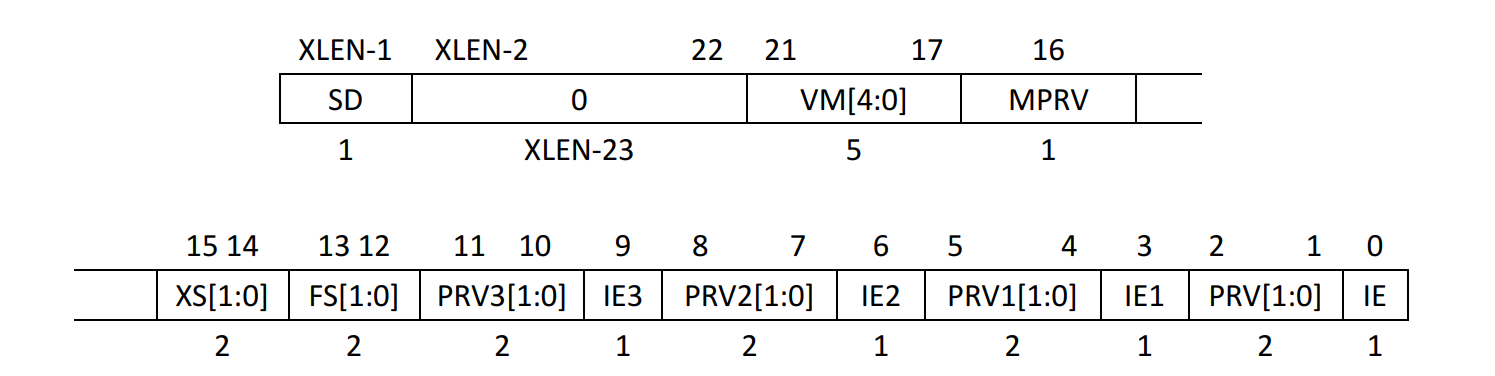
\includegraphics[width=0.8\textwidth]{mstatus.png}
    \caption{状态寄存器位域信息}
    \label{fig:mstatus}
\end{figure}

以状态寄存器CSR\_MSTATUS为例.如图~\ref{fig:mstatus}所示,mstatus 寄存器是一个XLEN位的可读/可写寄存器,其格式如图所示。mstatus 寄存器持续跟踪和控制硬件线程的当前操作状态。在写status寄存器的过程中,需要检查VM,MPP,MPRV,PUM,MXR位是否有变化,如果上述的位域发生改变,表示处理器状态发生改变,需要在寄存器读写之前判断当前特权等级。


如图是汇编指令mret的定义以及功能函数实现。
\begin{lstlisting}
    require_privilege(PRV_M);
    set_pc(p->get_state().mepc);
    reg_t s = STATE.mstatus;
    reg_t prev_prv = get_field(s, MSTATUS_MPP);
    s = set_field(s, MSTATUS_UIE << prev_prv, get_field(s, MSTATUS_MPIE));
    s = set_field(s, MSTATUS_MPIE, 1);
    s = set_field(s, MSTATUS_MPP, PRV_U);
    p->set_privilege(prev_prv);
    p->set_csr(CSR_MSTATUS, s);
\end{lstlisting}

在set\_csr()接口的实现中,需要对于CSR的读写进行检查,一方面是为了确保读写时所处的特权级模式是否支持读写,另一方面需要针对状态寄存器的改变做出相应的动作,比如tlb的清除等.
\begin{lstlisting}
case CSR_MSTATUS:
{
    if ((val ^ CSR.mstatus) & (MSTATUS_VM | MSTATUS_MPP | MSTATUS_MPRV | MSTATUS_PUM | MSTATUS_MXR))
        mmu->flush_tlb();
    reg_t mask = MSTATUS_SIE | MSTATUS_SPIE | MSTATUS_MIE | MSTATUS_MPIE
                | MSTATUS_SPP | MSTATUS_FS | MSTATUS_MPRV | MSTATUS_PUM
                | MSTATUS_MPP | MSTATUS_MXR ;
    if (validate_vm(max_xlen, get_field(val, MSTATUS_VM)))
    mask |= MSTATUS_VM;
    CSR.mstatus = (CSR.mstatus & ~mask) | (val & mask);
    bool dirty = (CSR.mstatus & MSTATUS_FS) == MSTATUS_FS;
    dirty |= (CSR.mstatus & MSTATUS_XS) == MSTATUS_XS;
    if (max_xlen == 32)
        CSR.mstatus = set_field(CSR.mstatus, MSTATUS32_SD, dirty);
    else
        CSR.mstatus = set_field(CSR.mstatus, MSTATUS64_SD, dirty);
    xlen = max_xlen;
    break;
}
\end{lstlisting}

除了上述的寄存器,每个处理器对象都维护私有的PC程序计数器,初始化过程中PC被初始化为bootrom地址.

\subsection{MMU和缓存模拟}

内存管理单元(Memory Management Unit, MMU)是一种负责处理CPU内存访问请求的计算机硬件。它的功能包括虚拟地址到物理地址的转换(即虚拟内存管理)、内存保护、中央处理器高速缓存的控制等。
\begin{figure}[h]
    \centering
    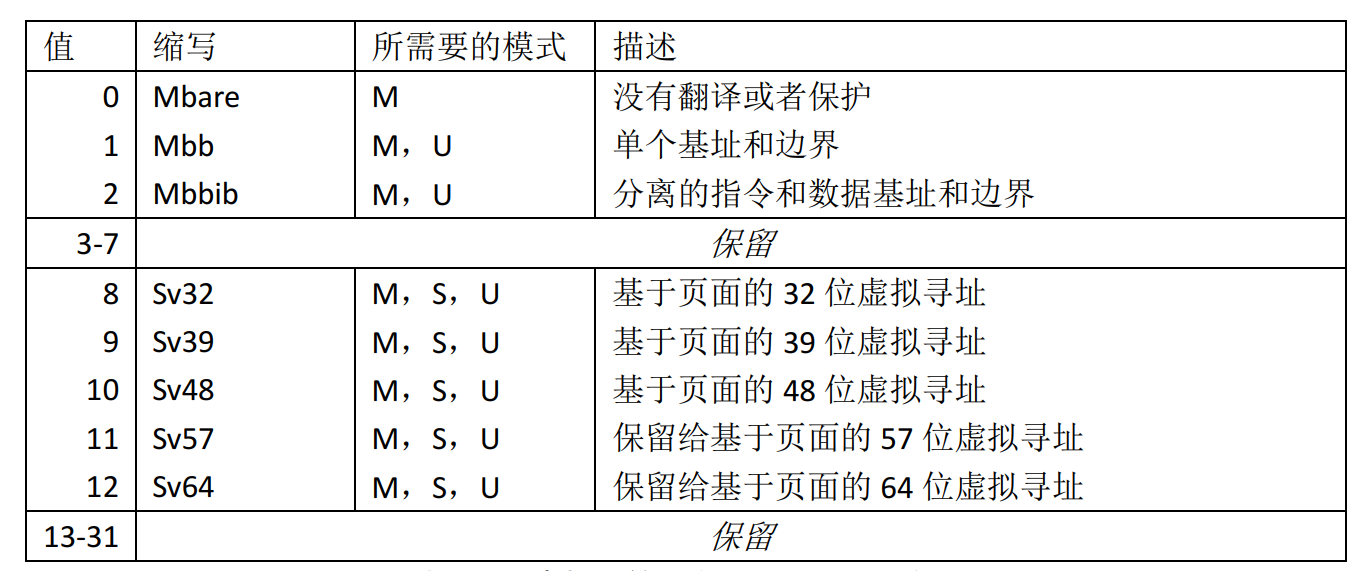
\includegraphics[width=0.8\textwidth]{VM.png}
    \caption{RISC-V虚拟化方案}
    \label{fig:VM}
\end{figure}

在RISC-V体系结构中,与MMU有关的CSR寄存器主要有控制与状态寄存器mstatus和管理员页表基址寄存器sptbr.在mstatus状态寄存器中,虚拟化管理字段 VM[4:0]指示了当前活跃的虚拟化方案,包括虚拟存储器翻译和保护。图~\ref{fig:VM}给出了当前定义好的虚拟化方案。对于一个 RISC-V 硬件实现,只有 Mbare 模式是强制要求的,该模式没有存储器管理或翻译,因此所有的有效地址,无论其特权模式,都被认为是机器物理地址,是复位时进入的模式,理论上在该模式下不需要经过MMU进行地址翻译。Sv39 和 Sv48 是针对 RV64 系统的基于页面的虚拟存储器体系结构,提供了一个 39 位或 者 48 位的虚拟地址空间,被设计成支持现代管理员级操作性,包括基于 Unix 的系统。Sv39、 Sv48 需要实现支持 M、 S 和 U 特权级。本模拟器支持上述三种虚拟化方案,但是为了实现方便,所有的主存访问请求都需要经过MMU,通过MMU模块的统一接口进行访存,当mstatus寄存器VM位为0时,无需进行地址翻译.以linux内核加载过程中从物理地址向虚拟地址过渡的逻辑可以看出,当内核支持MMU时,会进入到relocate代码段进行页表基地址寄存器的初始化,以后首级页表会常驻内存,内核通过setup\_vm()函数进行了首级页表的加载,然后在relocate段计算了首级页表基地址,写入sptbr寄存器,然后通过一条mret指令跳转到U-mode执行,接下来就全是加载虚拟地址了,MMU开始工作.
\begin{lstlisting}{}
    #ifdef CONFIG_MMU
    relocate:
        li a1, PAGE_OFFSET
        la a2, _start
        sub a1, a1, a2
    add ra, ra, a1
    
        la a2, 1f
        add a2, a2, a1
        csrw CSR_TVEC, a2
    
        srl a2, a0, PAGE_SHIFT
        li a1, SATP_MODE
        or a2, a2, a1
    
        la a0, trampoline_pg_dir
        srl a0, a0, PAGE_SHIFT
        or a0, a0, a1
        sfence.vma
        csrw sptbr, a0
    .align 2
    1:
        /* Set trap vector to spin forever to help debug */
        la a0, .Lsecondary_park
        csrw CSR_TVEC, a0
    
        /* Reload the global pointer */
    .option push
    .option norelax
        la gp, __global_pointer$
    .option pop
    
        csrw sptbr, a2
        sfence.vma
    
        ret
    #endif /* CONFIG_MMU */    
\end{lstlisting}


在本模拟器的实现中,MMU模块包含了快表TLB,加速地址翻译,本质上就是开辟了一片内存用来存放翻译过的地址映射,为了方便起见,只实现了直接映射的TLB.另外,将iCache,dCache的功能也一并放到MMU模块中,不再实现单独的缓存硬件模块,缓存采用只写的方式.这样的设计和真实硬件的差异很大,会导致缓存模拟的不准确.考虑到本模拟器并不进行缓存相关的性能模拟,所以可以忽略这部分的差别,在功能模拟上没有影响.模拟器的存储结构模型如图1.1所示.


MMU模块对取值做特殊处理,取值首先会查找iCache,当iCache未命中时,退化为其余类型的访存.访存请求通过模板函数提供的统一的接口load/store进行请求,通过模板可以忽略具体的数据类型,在功能函数的实现中也可以更加方便的使用,直接调用MMU的接口对存储单元进行操作.模板函数定义如下:
\begin{lstlisting}{}
    template<class T>
    inline T load(reg_t addr)
    {
        if (addr & (sizeof(T)-1))
            throw trap_t(trap_load_address_misaligned,addr);
        reg_t vpn = addr >> PGSHIFT;
        if (likely(tlb_load_tag[vpn % TLB_ENTRIES] == vpn))
            return *(T*)(tlb_data[vpn % TLB_ENTRIES] + addr);
        T res;
        load_slow_path(addr, sizeof(T), (uint8_t*)&res);
        return res;
    }    
\end{lstlisting}


其中,load\_slow\_path()意味着TLB miss,需要查找页表,通过页表进行地址翻译的伪代码如图所示:


综上,整个MMU和缓存模块的实现流程如图~\ref{fig:mmu-cache}所示.


\subsection{总线和I/O模拟}
总线是CPU与外部设备进行数据交换的桥梁,按照功能划分可以分为地址总线,数据总线和控制总线.本模拟器对总线设备进行了抽象,将总线设计为某一块物理地址区间内的IO控制器,提供统一接口,处理CPU和内存映射的IO设备之间的通信.


总线在模拟器初始化的过程中会根据配置挂载设备,在总线类bus\_t中维护一个物理地址和设备类对象的map,模拟器在接收到访存请求时,首先检查物理地址是否是主存地址范围,不在主存地址区间内的I/O请求都是内存映射的I/O请求(Memory-Mapped I/O, MMIO),模拟器将调用总线设备的IO接口,对内存映射的外设进行读写操作.
\begin{figure}[h]
    \centering
    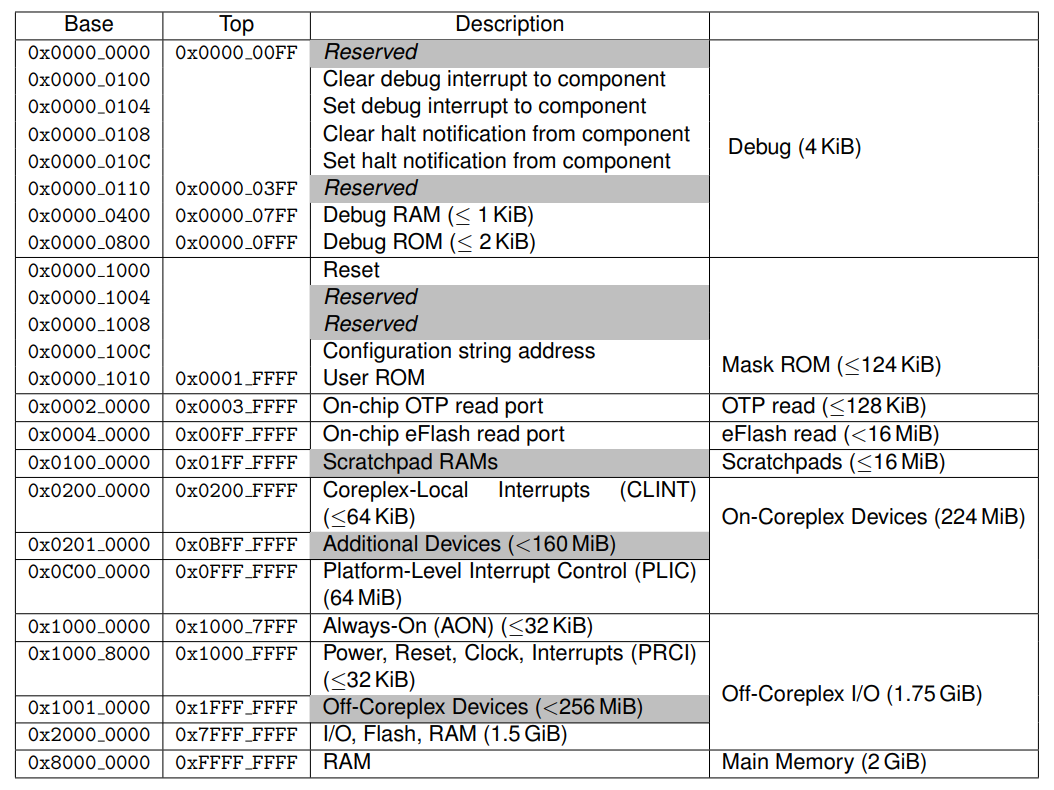
\includegraphics[width=0.8\textwidth]{mmap.png}
    \caption{SiFive公司的内存映射方案}
    \label{fig:mmap}
\end{figure}

模拟器根据物理地址划分为主存,和内存映射的IO设备,图~\ref{fig:mmap}是SiFive公司提供的内存映射参考.本模拟器的总线设备需要处理的内存映射空间就是0x00000000~0x80000000,提供这块内存区间上的IO模拟.总线设备可以挂载各种通过内存映射的IO设备,某些具有特殊用途的寄存器也能够挂载在总线,比如timecmp寄存器,ipi寄存器.


总线设备的定义如下:
\begin{lstlisting}{}
    class bus_t : public abstract_device_t
    {
    public:
        bool load(reg_t addr, size_t len, uint8_t* bytes);
        bool store(reg_t addr, size_t len, const uint8_t* bytes);
        void add_device(reg_t addr, abstract_device_t* dev);
        void add_register(reg_t addr, abstract_device_t* dev,qint32 offset);
    
    private:
        std::map<reg_t, abstract_device_t*> devices;
        struct device_reg
        {
            device_reg(){}
            device_reg(abstract_device_t *dev,qint32 offset):dev(dev),offset(offset){}
            abstract_device_t *dev;
            qint32 offset;
        };
        QMap<reg_t,device_reg> regs;
    };     
\end{lstlisting}

bus\_t类型的load/store属于mmio接口,首先会检查挂载在总线上的设备或寄存器地址是否匹配,然后才会对具体的设备进行读写操作.


下面介绍几种以MMIO方式挂载在总线上的设备模拟.


所有支持Secure Boot的CPU都会有一个bootrom固件.CPU 在通电之后执行的第一条指令就在 bootROM 的入口。bootROM 拥有最高的执行权限,也就是机器模式M-mode。它将初始化 Secure Boot安全机制,加载 Secure Boot Key 等密钥、从存储器加载并验证First Stage Bootloader(FSBL),最后跳转进 FSBL中。本次芯片设计项目也包含了该部分的设计,但是由于涉密,在模拟器设计中并不涉及FSBL的加载和验证过程,bootrom固件程序仅仅用来跳转置目标程序入口.具体的实现方式包括以下的步骤,首先在配置中读取bootrom的地址,默认0x1000,然后初始化bootrom设备,填写bootrom固件内容,本模拟器的bootrom程序内容如图所示,包含两条汇编指令:\\
auipc	t0, 0x7ffff\\
jr 	t0\\
模拟器启动后,PC初始化0x1000,以机器模式执行上述两条指令,跳转到主存起始位置,即目标程序的入口地址.接下来的一系列指令执行由目标程序决定,主要包括bootloader的reset vector以及加载linux内核的过程.


总线对象使用add\_device接口将物理地址0x1000和bootrom设备对象的映射保存在字典中.


mmio的通信流程如图~\ref{fig:mmio}所示.
\begin{figure}[h]
    \centering
    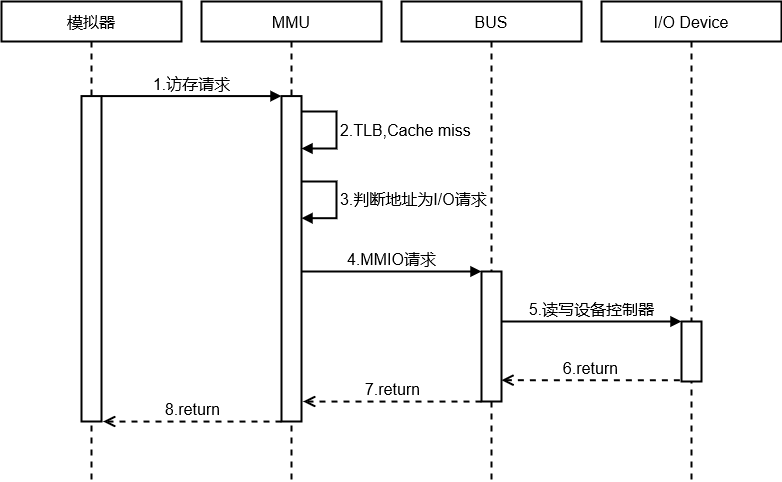
\includegraphics[width=0.8\textwidth]{mmio.png}
    \caption{MMIO请求流程}
    \label{fig:mmio}
\end{figure}


\section{中断系统的实现}

在CPU运行过程中,存在两种指令流程,一种是常规的逻辑控制流,包括顺序的指令流和分支跳转;另一种称为异常控制流,用来响应处理器状态的某些变化,表现为中断或异常.之前的章节已将介绍了CPU指令控制流程的模拟,其中包括了响应中断的逻辑,CPU在取值之前检查当前是否有中断信号,根据状态寄存器判断是否响应中断,进入异常控制流逻辑.本节将详细阐述模拟器中断系统的实现.包括两种中断控制器以及部分中断源的模拟.


RISC-V一共有两大类的中断类型:局部中断(Local Interrupts)以及全局中断(Global Inerrupts)。局部中断是指直接与hart相连的中断,可以直接通过CSRs当中的xcause(mcause、scause、ucause)中的值得知中断的类型。在局部中断当中,只有两种标准的中断类型:计时中断(timer)以及软件中断(software)。全局中断实际上就是外部中断(External Interrupts)。它与PLIC相连(Platform-Level Interrupt Controller,平台级中断控制器)。实际上全局中断在多个硬件线程的情况下最为常用。PLIC用于对外部中断进行仲裁,然后再将仲裁的结果送入核内的中断控制器。
RISC-V 架构中规定了一些硬件行为来实现异常事件的响应和处理,这些行为通过控制状态寄存器来反应异常事件信息.涉及到如下几个寄存器,见表~\ref{tab:csr}.
\begin{table}[h]
  \centering
  \caption{中断相关的寄存器}
  \label{tab:csr}
  \begin{tabular}{cl}
    \toprule
寄存器	& \multicolumn{1}{c}{功能}\\
    \midrule
    mstatus	& \multicolumn{1}{m{9cm}}{状态寄存器,保存全局中断使能以及许多其他的状态。只讨论机器模式的情况下,有效的域只有 MIE 和 MPIE。MIE 表示中断全局使能,只有该位有效时,才能产生中断。MPIE位保存进入中断处理之前以及恢复现场之前 MIE 的状态。}\\ \hline
    mie	& \multicolumn{1}{m{9cm}}{外部中断使能寄存器,外部中断响应的使能位有效时才能进入处理}\\ \hline
    mtvec	& \multicolumn{1}{m{9cm}}{异常入口基地址寄存器,可配置为查询或向量访问模式。高位BASE 域表示异常向量的基地址。}\\ \hline
    mscratch & \multicolumn{1}{m{9cm}}{上下文切换时用于保存当前的指针信息}\\ \hline
    mepc & \multicolumn{1}{m{9cm}}{异常 PC 寄存器,进入中断处理时,硬件会自动将当前遇到的中断的 PC 保存 mepc 中}\\ \hline
    mcause & \multicolumn{1}{m{9cm}}{异常原因寄存器,mcause[31]为中断域,其余位为异常编号域。如果是有中断事件待处理,会将 interrupt 位置 1。Exception Code 字段保存待处理事件的标识代码。中间位读时返回 0,作为保留位可以在之后用于支持异常编码的字段扩展}\\ \hline
    mip	& \multicolumn{1}{m{9cm}}{外部中断事件标志信号,当有外部中断事件发生时,mip中对应中断标志位置高}\\ \hline
    mbadaddr & \multicolumn{1}{m{9cm}}{外部中断事件标志信号,当有外部中断事件发生时,mip中对应中断标志位置高}\\
    \bottomrule
  \end{tabular}
\end{table}

本模拟器实现了这部分的硬件行为,包括中断源的产生,和中断响应,下面进行详细的介绍.在处理器类内定义了两个uint64型数据,分别用来表示时钟中断和外部中断的pending,总线上挂载的设备可以直接对这两个pending数据进行设置,用来模拟外设”异步”的中断请求发起.处理器在下一个取值周期之前,使用try-catch语句来处理可能的中断响应,如果处理器决定响应中断,就会抛出一个trap\_t类型的异常,进入到响应中断的异步逻辑.trap\_t的定义如下:
\begin{lstlisting}{}
    class trap_t
    {
    public:
        trap_t(){}
        trap_t(reg_t type):cause(type),addr_valid(false){}
        trap_t(reg_t type,quint64 addr):cause(type),addr_valid(true),addr(addr){}
        reg_t cause;
        bool addr_valid;
        quint64 addr;
        static QMap<reg_t,QString> names;
        static quint64 delegable_exceptions;
        QString &name(){return names[cause];}
    };        
\end{lstlisting}

处理器响应的流程如图~\ref{fig:interrupt}所示.
\begin{figure}[h]
    \centering
    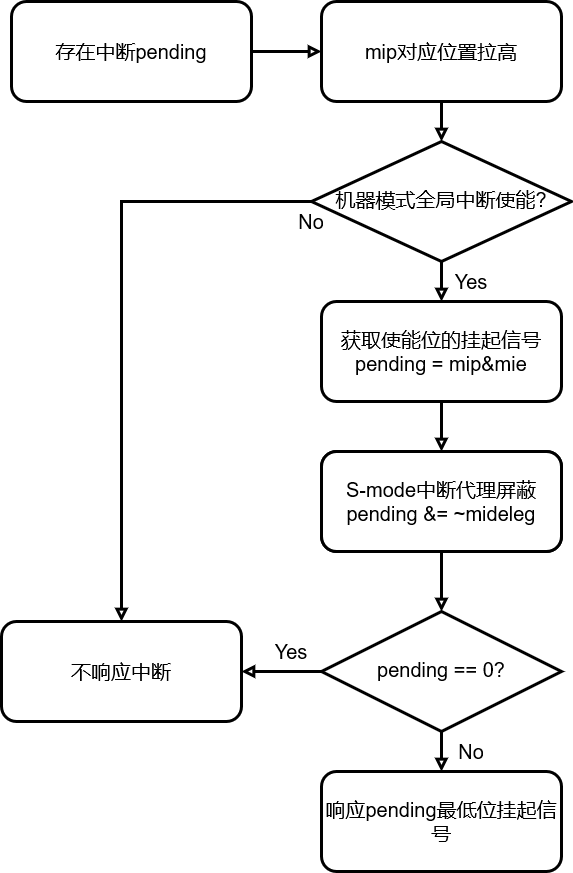
\includegraphics[width=0.6\textwidth]{interrupt.png}
    \caption{处理器响应中断流程}
    \label{fig:interrupt}
\end{figure}

模拟器抛出异常后,根据捕获到的trap\_t,进入中断处理流程.RISC-V特权架构对这部分的处理器行为做了一定规范,本模拟器的实现也参照了特权架构定义.


1) 根据处理的中断类型将信号源编号记录到mcause寄存器中;


2) 地址不对齐或者发生访问异常,将导致错误的指令部分保存到mbadaddr;


3) 更新状态寄存器mstatus,记录中断处理前的状态;


4) 保存当前PC到 mepc寄存器中,以便于处理完中断后返回;


5) 停止当前执行程序流,设置PC为mtvec中断向量表入口地址并开始执行.


以上就是中断产生和响应过程对应的处理器硬件行为模拟,接下来将着重阐述平台级中断控制器PLIC的实现.


\subsection{PLIC模拟}

PLIC的功能是接受外部中断源发出的中断信号,对中断请求进行裁决,将裁决结果和外部中断信号发送给处理器.本模拟器参照了SiFive公司的PLIC规范文档进行设计,通过设备树的挂载对内存映射的存储器进行读写,配置PLIC.


图~\ref{fig:plic-core}是SiFive公司给出的PLIC规范框架图.
\begin{figure}[h]
    \centering
    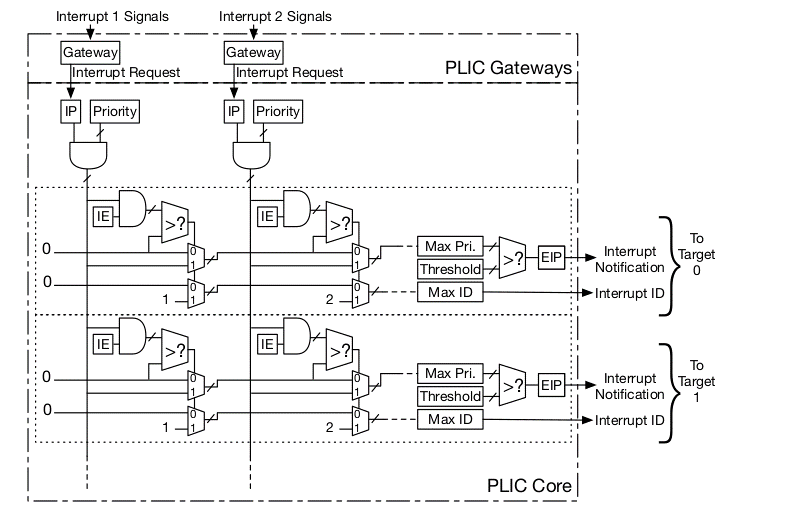
\includegraphics[width=0.8\textwidth]{plic-core.png}
    \caption{SiFive公司的PLIC框架}
    \label{fig:plic-core}
\end{figure}


中断源(interrupt sources)是挂载在PLIC上的设备的统称,一般是I/O设备.PLIC理论上支持任意多个中断源,每个中断源可以是不同触发类型,电平触发或者边沿触发、PLIC为每个中断源分配了如下的信息:


1) 闸口(Gateway)和IP(interrupt pending).闸口控制中断源发送中断请求.IP标识当前中断源是否有请求.IP拉高时,闸口不再接受该中断源的请求.


2) 设备编号ID.PLIC为每个中断源分配了一个独一无二的编号ID.该ID也作为在多个sources具有相同优先级是的选择条件,数值较小优先级更高。


3) 优先级(Priority).每个中断源都有一个内存映射的Priority寄存器,表示该中断源的优先级,软件可以通过配置(设备树)将其设置成不同的优先级.优先级的数字越大,表示优先级越高.


中断使能(Enable).每个中断源均分配了一个内存映射的中断使能寄存器,和优先级一样也可以通过设备树进行配置.IE寄存器配置为0表示该中断源被中断目标屏蔽,反之则是使能.


中断目标(interrupt targets)对应为RISC-V处理器核心的各个特权级模式。PLIC产生的外部中断请求会分别标示在处理器的mip寄存器的meip/seip位,对应于机器模式和监管模式。每个中断目标都有对应的内存映射的优先级门限(priority threshold)寄存器,只有中断源优先级高于该门限,PLIC才会将中断源ID发送给对应中断目标。


PLIC Core负责所有中断请求的仲裁和分发.图~\ref{fig:plic-process}展示了PLIC处理外部中断的流程.
\begin{figure}[h]
    \centering
    
\includegraphics[width=0.8\textwidth]{plic-process.png}
    \caption{PLIC中断处理流程}
    \label{fig:plic-process}
\end{figure}

将中断源和中断目标分别抽象成plic\_dev\_info\_t类和plic\_core\_info\_t类,在外设模拟中,通过connect\_plic接口初始化设备类中的plic\_dev\_info\_t对象,并将自身挂载到PLIC设备上,后续设备的IO请求可以通过plic\_dev\_info\_t::raise()接口发送到PLIC设备,模拟了闸口的功能.PLIC设备类型plic\_t中定义了accept\_interrupt接口用来拉高对应设备的pengding寄存器,plic\_t::raise()接口实现了中断信号裁决,将裁决后的中断ID写入mclaim和sclaim寄存器,并且向处理器发送外部中断信号,当处理器响应中断时,会读取这两个寄存器的值,然后进入中断向量表,查找对应的中断处理函数,通常会调用定义在内核drives目录下的驱动程序.中断处理结束后,处理器会给PLIC core发送中断完成信息,具体的动作就是对PLIC中断源指定位置claim寄存器发送一条store指令,根据SiFive公司给出的规范,中断源ID为n的的claim/complete寄存器内存映射位置等于(plic基地址+0x200004+0x1000*n),因此该位置进行store请求时直接调用处理器对应plic\_core\_info\_t对象的gate\_open()接口来打开闸口.此时plic完成一次外部中断请求周期,可以挂起下一次的中断请求.


根据以上的流程,实现PLIC中断控制器的设备类图如图~\ref{fig:plic-class}所示。
\begin{figure}[h]
    \centering
    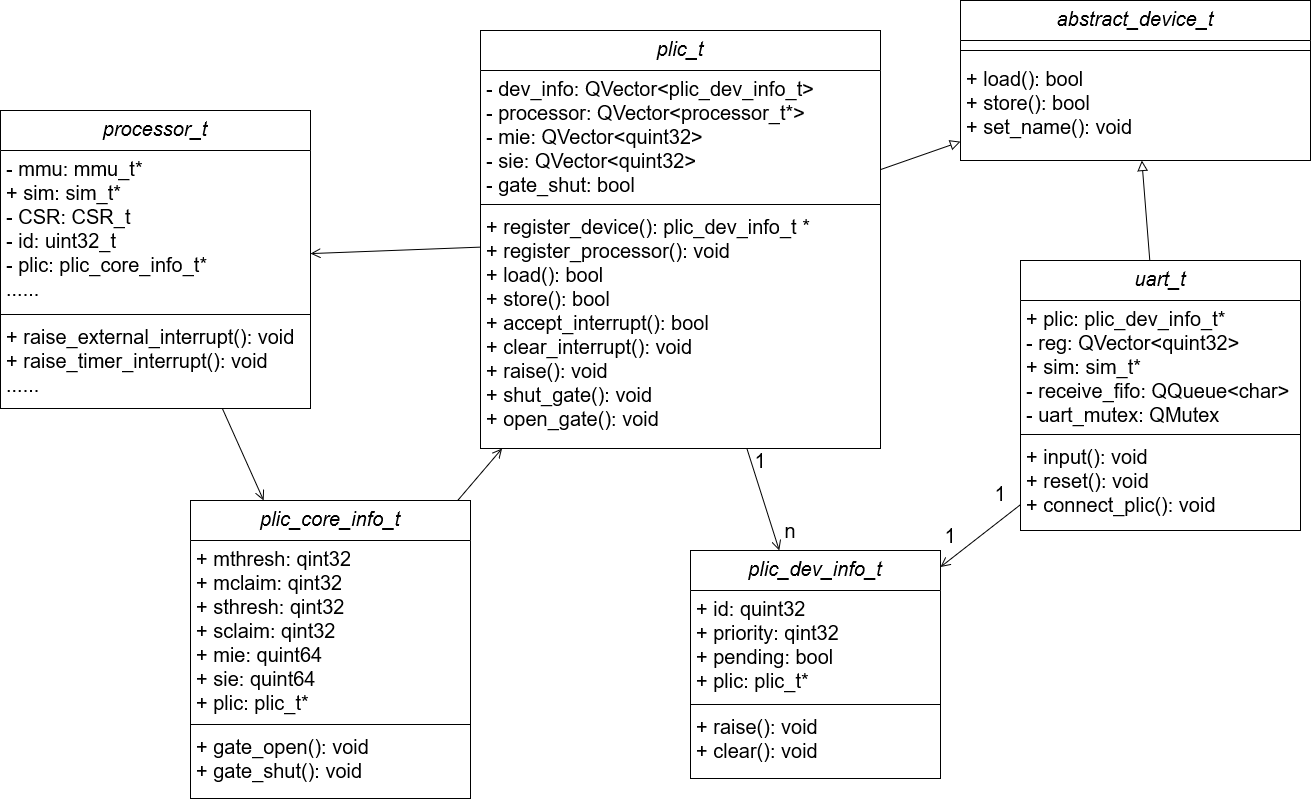
\includegraphics[width=0.8\textwidth]{plic-class.png}
    \caption{PLIC设备类图}
    \label{fig:plic-class}
\end{figure}


\subsection{RTC模拟}

CLINT(Core-Local Interruptor, PLIC)局部中断控制器是一个存储器地址映射模块,CLINT只负责处理软件中断和时钟中断,因为这两个中断是RISC-V架构中定义的,经过CLINT不需要进行任何的仲裁,直接将中断信号写入对应的寄存器内即可。软件中断只需要向CLINT的MSIP0或者SSIP0寄存器的最高位写1即可,处理完中断后,将其置为0,这样就能够清除掉软件中断的标志位。计时器中断作为riscv内核特有的中断,其用法就是往MTIMECMP或者STIMECMP中写特定的值,当mtime达到该值时产生中断,此时继续填写特定的tick就可以继续产生下个中断,反复如此,便可产生周期性的tick中断。

% \subsection{外部中断源模拟}


\section{调试模块和UI实现}
调试模块能够提供断点设置,单步执行,寄存器/内存查询等功能.UI显示界面主要包含了断点设置窗口,查询窗口和执行交互窗口.本模块使用Qt的UI Designer工具进行开发,通过拖拽摆放各种窗口控件并进行属性设置,观察界面整体效果,可以方便地进行可视化界面的设计.另外QtWidget库还提供了信号(Signals)和槽(Slots)机制,用于对象间通信,只需要在对应窗口子类化widgets来添加自定义信号,然后实现自定义的槽函数,连接到该信号即可.


模拟器前端整体界面如图~\ref{fig:zhenti}所示.
\begin{figure}[h]
    \centering
    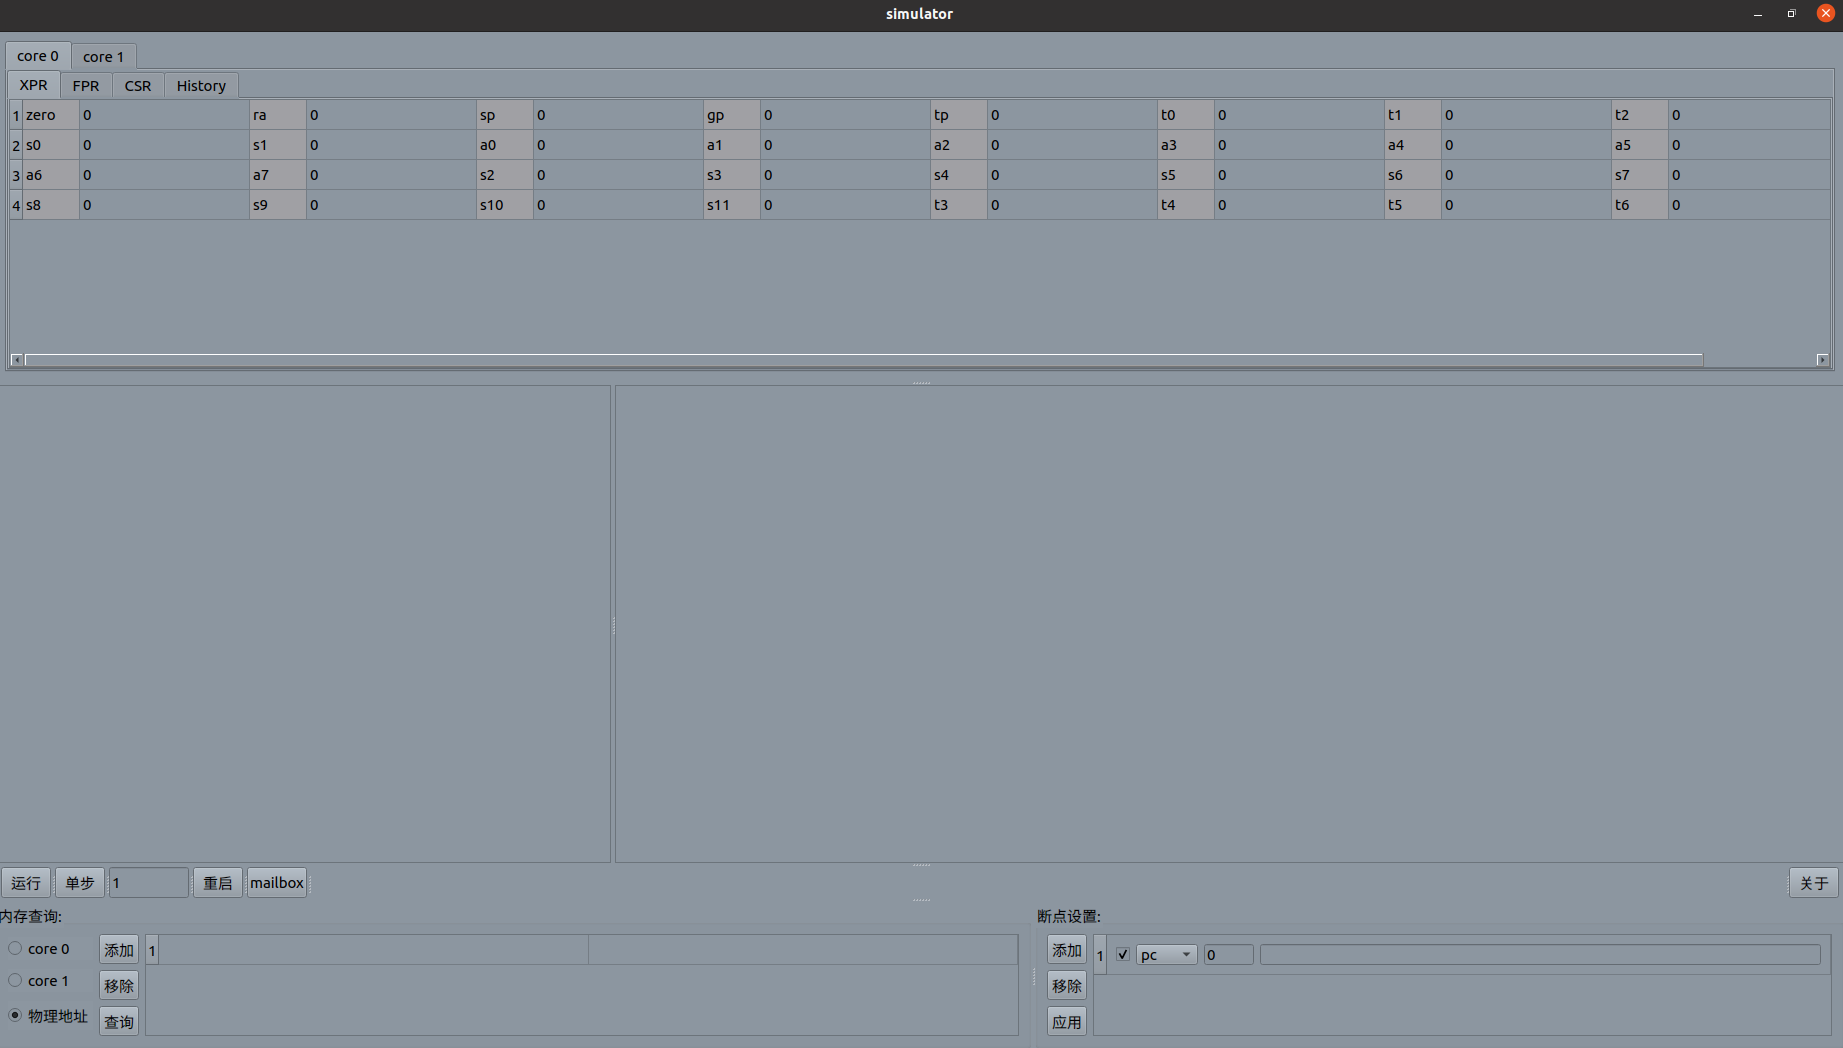
\includegraphics[width=1.0\textwidth]{zhenti.png}
    \caption{模拟器前端整体界面}
    \label{fig:zhenti}
  \end{figure}


前端UI窗口和后端模拟器之间的信号定义如下:
\begin{lstlisting}{}
    enum sim_cmd
    {
        sim_cmd_pause_sim,
        sim_cmd_run_sim,
        sim_cmd_run_sim_silently,
        sim_cmd_step_sim,
        sim_cmd_reset_sim,
        sim_cmd_access_memory,
        sim_cmd_set_breaks,
        sim_cmd_key_input,
        sim_cmd_mailbox_input
    };
    
    enum window_cmd
    {
        window_cmd_update_reg,
        window_cmd_update_mem,
        window_cmd_sim_output,
        window_cmd_gst_output,
        window_cmd_pause_sim,
        window_cmd_update_mailbox
    };          
\end{lstlisting}

其中sim\_cmd\_key\_input和sim\_cmd\_mailbox\_input信号分别用来模拟UART和mailbox外部中断源信号.其余信号用于断点和查询信息的交互,以及模拟器单步运行等流程的控制.


断点设置窗口如图所示,可以添加任意多个断点,断点匹配类型分为如下几种:PC,寄存器,内存,中断类型.当模拟器包含多核时需要指定相应的核心id号.当模拟器处于调试模式时,中断指令流程,此时可以进行断点设置,内存查询等操作,点击运行按键,模拟器恢复至正常运行模式,在每一次指令执行周期完成后模拟器将对当前断点信息进行检查,一旦匹配上任意断点,将发送window\_cmd\_sim\_output信号用于告知触发断点信息,并接着发送window\_cmd\_pause\_sim信号,中断指令流程,模拟器进入调试模式.每发送一次单步执行信号,模拟器都需要将寄存器更新信号发送给UI前端,刷新寄存器窗口.


模拟器单步执行的流程如图~\ref{fig:step}所示.
\begin{figure}[h]
    \centering
    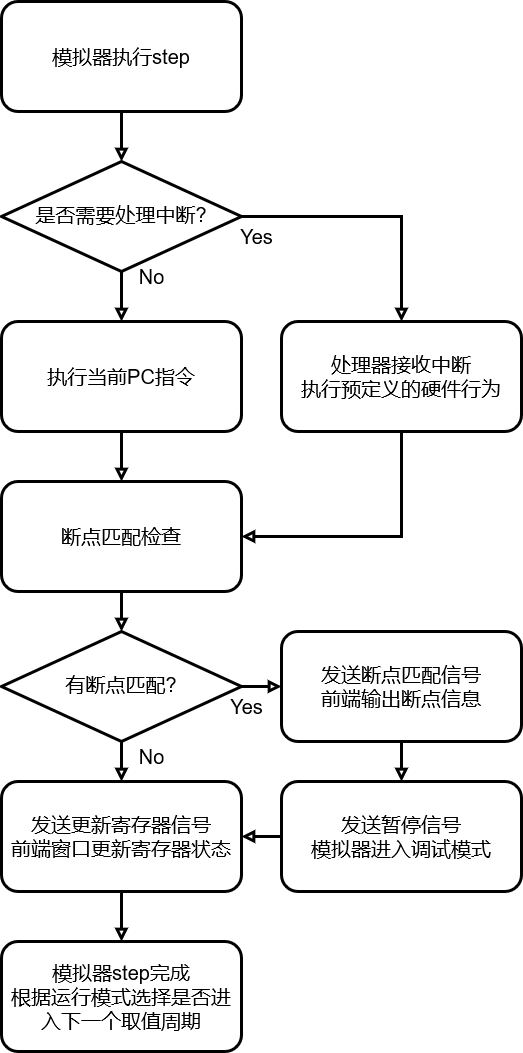
\includegraphics[width=0.4\textwidth]{step-logic.png}
    \caption{调试模式下单步执行流程}
    \label{fig:step}
\end{figure}


\section{本章小结}
本章主要在概要设计的基础上对RISC-V指令集模拟器四个功能模块的详细设计和实现细节进行了阐述,并根据实际工程项目中使用的设备和具体型号IP文档,进行了部分外设的功能模拟,验证了模拟器的可用性,最后完成了前后端所有功能模块的代码实现,并给出了相应的演示效果图.


